\chapter{Concepts to build Distributed Systems}

\section{Remote Procedure Calls}
Remote procedure calls are function calls that are not part of the main node, instead, the node calls another node running somewhere else and gets the result back. Consider the following system for an e-commerce website, that uses stripe for payment processing:

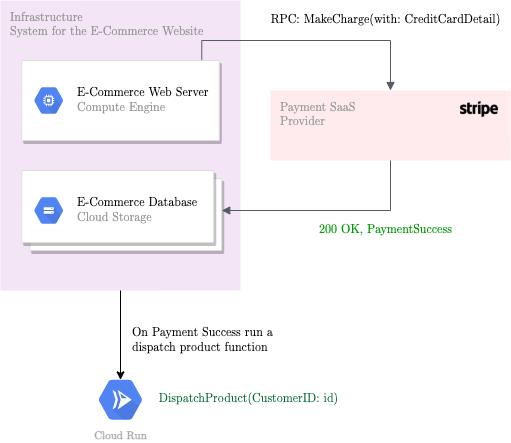
\includegraphics[scale=0.60]{images/RPC.png}

\noindent This e-commerce website is running on Google Cloud and calls \texttt{MakeCharge()} function call to stripe's server. This calling a function that is on a different node is called a remote procedure call.

\noindent This \texttt{MakeCharge()} function logic and implementation are handled by Stripe, they contact the VISA or MasterCard or RuPay server, those payment processors call the Bank to verify credentials and debits the money then VISA or MasterCard server calls stripe to say the payment is OK then stipe calls our e-commerce website that the payment is processed. The banks have different servers, the VISA, MasterCard companies have different servers, stripe as well as our e-commerce website are running on different servers.

\noindent This is the best thing about RPCs. We don't have to directly talk to the bank to debit money for the customers' accounts we will call some RPC and we don't have to handle the rest of the logic. These RPCs can call servers belonging to different companies or even the same companies owned by a different engineering team. This creates an abstraction of code and logic in our programs. In case the stripe server fails, our website remains unaffected for simple product browsing and virtually nothing happens to the customers ordering by cash on delivery.

\subsection{RPC marshalling}
\noindent To communicate with each other, the servers may need to make available a common message protocol. Let's say our web server is running \textbf{Flask} Python framework and Stripe uses Ruby and CoffeeScript according to \href{https://techstacks.io/stacks/stripe}{\textcolor{blue}{TechStack.io}}. So to communicate with each other stripe and our server must conform to some common message structure. In most cases nowadays we use REST-JSON format to communicate between servers.

\subsection{Problems with RPCs}
In the best-case scenario, all the RPC calls should behave like it's running inside the caller machine, but many problems may arise during RPC calls.

\begin{itemize}
    \item RPC \texttt{MakeCharge()} do not go through
    \item RPC \texttt{MakeCharge()} goes through but the stripe server fails during the execution of \texttt{MakeCharge()}
    \item \texttt{MakeCharge()} goes through but the \texttt{PaymentSuccess} message is lost or delayed and the e-commerce site to stripe connection times out. This is a bad scenario because the customer money is debited but the cloud run function call \texttt{DispatchProduct()} \textcolor{red}{will not run} because this function is run after the acknowledgement is store on the database.
    \item \texttt{PaymentSuccess} successfully comes back but the e-commerce server fails during the handling of a successful payment.
\end{itemize}

\section{Time, Clocks, Event Orders}
In distributed systems clocks are enormously important. Time plays a crucial role in the ordering of events. Some of the other things we need time for are the following

\begin{itemize}
    \item operating systems at several nodes need time to keep track of CPU usage, utilization, network latency,
    \item validate and store data with limited time validity [time-based caches]
    \item record when some event occurred
    \item determining the order of events in a several node architectures which we'll discuss below
\end{itemize}

Suppose there are three systems A, B, and C. Now \textbf{A} sends a message to B and C that \textit{hey, some systems are down in Europe please redirect to India}, hearing this \textbf{B} sends a message to A and C that \textit{No, Indian servers are also down, please redirect all Indian traffic as well as European traffic to North America}.

\noindent Now look from the American Server C's perspective. Due to network delay, it may happen that message from \textbf{B} arrives first before the message from \textbf{A}. This order doesn't make any sense for \textbf{C} right? If there is some way to order those messages... Oh, we can put some timestamp to each message, so that we can later decode what is the order of received messages and process those messages in their intended order.

\noindent But in distributed systems there is \textcolor{red}{no concept of \textbf{global time}}. Many times servers are running across different zones, we can sync time with that server using NTP (Network time protocol). For example, Apple has a network time server that can be reachable at \texttt{time.apple.com}. Once we find the time difference between the machine host and the time server the host machine gently adjusts time by running a little slower or faster on the machine to match with the time server. This gradually reduces the time difference over the course of a few minutes. If NTP finds the difference much more it may reject to change the time on a host and stop, leaving a human operator to adjust the clock.

\noindent For these above reasons timestamps can't be reliable in distributed systems. It may so happen that timestamp on message \textbf{A $\to$ (B and C)} $>$ timestamp on message \textbf{B $\to$ (A and C)}. Now the time delta becomes \textbf{-ve} meaning again the message ordering flipped.

\subsection{Physical Clocks and Logical Clocks}
There are 2 types of clocks in the distributed systems, one being physical which counts [how many] seconds elapsed and other being a logical clock which counts logical events like [number of communication happened, number of time a connection created or destroyed].